\documentclass{beamer}

\usepackage[utf8]{inputenc}
\usepackage{hyperref}

\usetheme{Berkeley}
\beamertemplatenavigationsymbolsempty
\setbeamertemplate{headline}{}
 
\title{Geocoding mit Photon in FoodChain-Lab}
%\subtitle{Geocoding with Photon}
\date{}
 
\begin{document}
\maketitle

\section{ }

\subsection{Aufgaben}
\begin{frame}
	\begin{itemize}
		\item Führen Sie ein Geocoding auf Basis folgenden Workflows durch: \url{https://github.com/SiLeBAT/BfROpenLabResources/raw/master/GitHubPages/workflows/Geocoding_with_Photon.knwf}.
		\item Fügen Sie den \textbf{FoodChain-Lab} \textbf{Geocoding} Knoten hinzu.
		\item Verwenden Sie den Photon Geocoding Service.
	\end{itemize}
\end{frame}
 
\subsection{1}
\begin{frame}
	\begin{center}
  		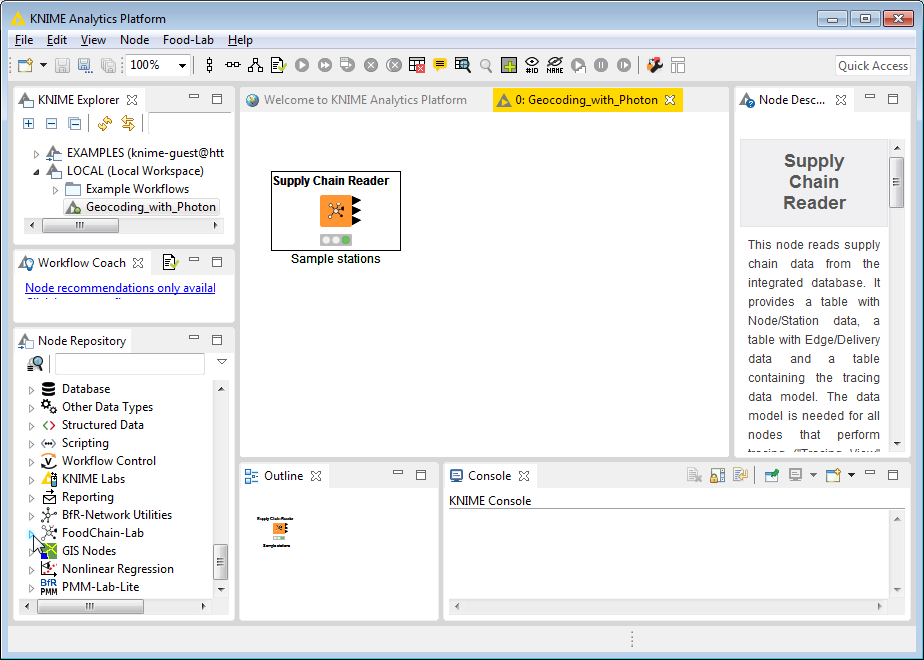
\includegraphics[height=0.6\textheight]{1.png}
	\end{center}
	\begin{itemize}
		\item Importieren Sie den Geocoding Workflow von \url{https://github.com/SiLeBAT/BfROpenLabResources/raw/master/GitHubPages/workflows/Geocoding_with_Photon.knwf}.
		%\item In this tutorial we are using the Photon Geocoding service.
	\end{itemize}
\end{frame}

\subsection{2}
\begin{frame}
	\begin{center}
  		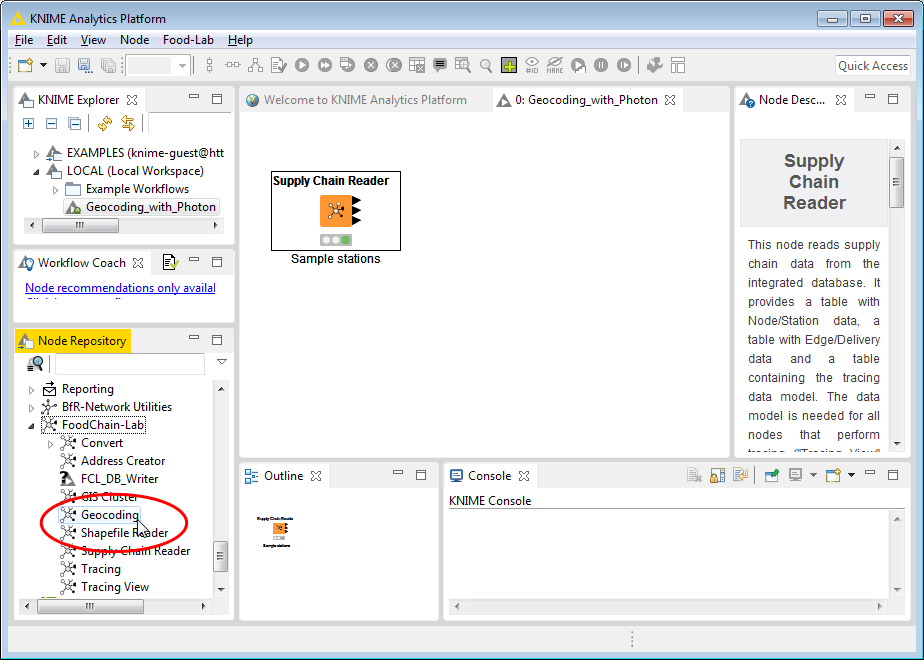
\includegraphics[height=0.6\textheight]{2.png}
	\end{center}
	\begin{itemize}
        \item Um den Geocoding Service zu nutzen muss der \textbf{FoodChain-Lab} \textbf{Geocoding} Knoten hinzugefügt werden.
		\item Fügen Sie den \textbf{FoodChain-Lab} \textbf{Geocoding} Knoten hinzu durch einen Doppelklick darauf im \textbf{Node Repository}.
		%\item In this tutorial we are using the Photon Geocoding service.
	\end{itemize}
\end{frame}

\subsection{3}
\begin{frame}
	\begin{center}
  		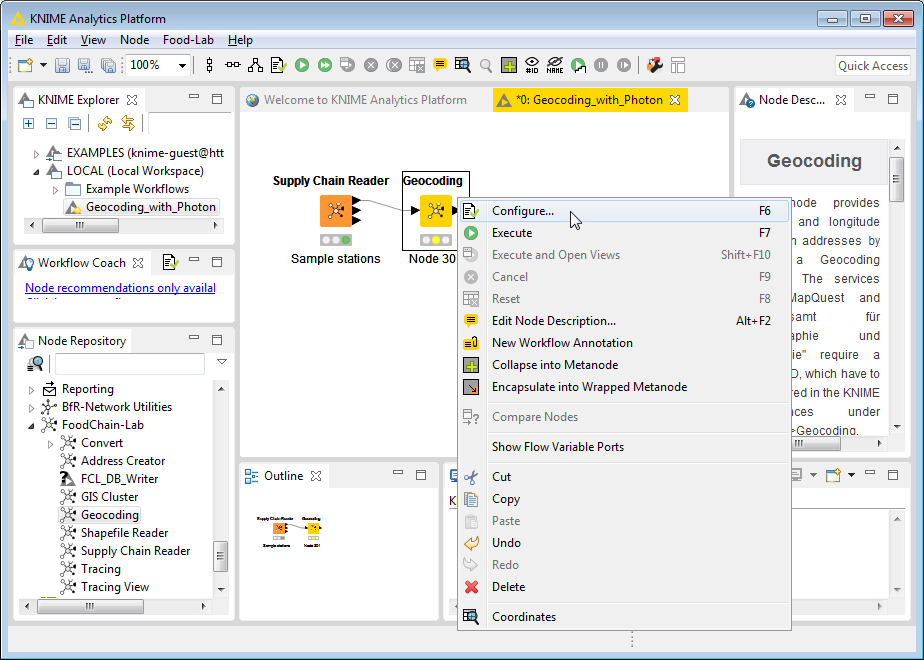
\includegraphics[height=0.6\textheight]{3.png}
	\end{center}
	\begin{itemize}
        \item Ein \textbf{Geocoding} Knoten wurde zum Workflow hinzugefügt. Er ist verbunden mit dem \textbf{SupplyChainReader} und muss konfiguriert werden.
		%\item The \textbf{Geocoding} node has to be set up (to use Photon)
		\item Öffnen Sie den Konfigurationsdialog durch einen Doppelklick auf den Knoten oder durch Benutzung des Kontextmenüs (Rechtsklick auf den Knoten).
		%\item In this tutorial we are using the Photon Geocoding service.
	\end{itemize}
\end{frame}

\subsection{4}
\begin{frame}
	\begin{center}
  		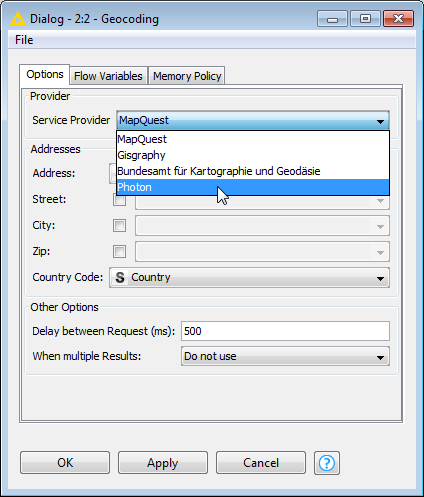
\includegraphics[height=0.6\textheight]{4.png}
	\end{center}
	\begin{itemize}
        \item Setzen Sie den \textbf{Service Provider} auf \textbf{Photon}.
		%\item The Geocoding-Node has to be configured (to use Photon)
		%\item Open its configuration by double clicking on it or by using its context menue (right click on the node)
		%\item In this tutorial we are using the Photon Geocoding service.
	\end{itemize}
\end{frame}

\subsection{5}
\begin{frame}
	\begin{center}
  		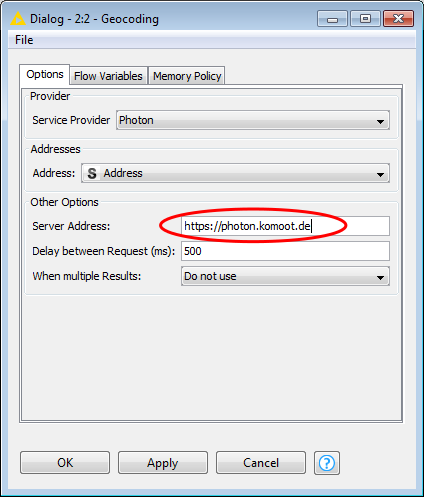
\includegraphics[height=0.6\textheight]{5.png}
	\end{center}
	\begin{itemize}
        \item Die \textbf{Address} ist passend gesetzt.
		\item Sie müssen die \textbf{Server Address} eingeben. Dafür können Sie \textbf{http://photon.komoot.de} nutzen, einen öffentlich verfügbaren Dienst. 
		%\item The Geocoding-Node has to be configured (to use Photon)
		%\item Open its configuration by double clicking on it or by using its context menue (right click on the node)
		%\item In this tutorial we are using the Photon Geocoding service.
	\end{itemize}
\end{frame}

\subsection{6}
\begin{frame}
	\begin{center}
  		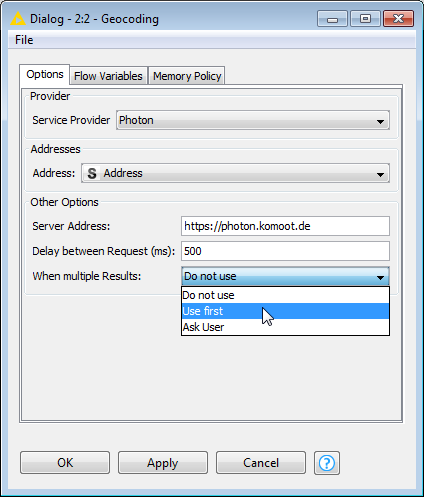
\includegraphics[height=0.5\textheight]{6.png}
	\end{center}
	\begin{itemize}
		\item Es passiert häufig, dass der Geocoding Service zu einer Anfrage mehrere Resultate liefert (z.B. wenn es mehrere Straßen mit demselben Name in einer Stadt gibt).
		\item Wir müssen definieren was in diesem Fall passieren soll: kein Resultat nehmen, das erste Resultat nehmen oder das passende Resultat manuell auswählen.
		\item Manuelles Auswählen ist bei großen Datenmengen sehr arbeitsaufwendig, deshalb wählen wir hier einfach \textbf{Use first} und klicken \textbf{OK}.
	\end{itemize}
\end{frame}

\subsection{7}
\begin{frame}
	\begin{center}
  		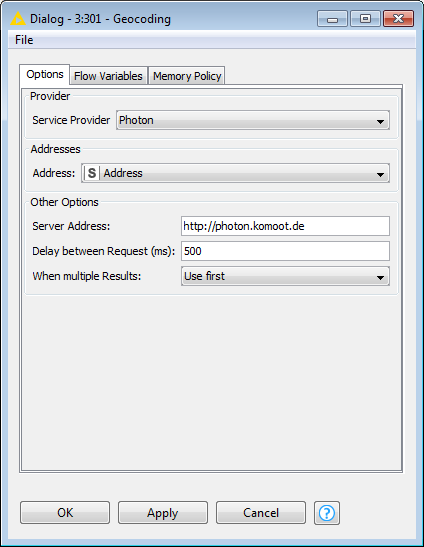
\includegraphics[height=0.6\textheight]{7.png}
	\end{center}
	\begin{itemize}
		\item Machen Sie einen Rechtsklick auf den \textbf{Geocoding}-Knoten und wählen Sie \textbf{Execute}.
	\end{itemize}
\end{frame}

\subsection{8}
\begin{frame}
	\begin{center}
  		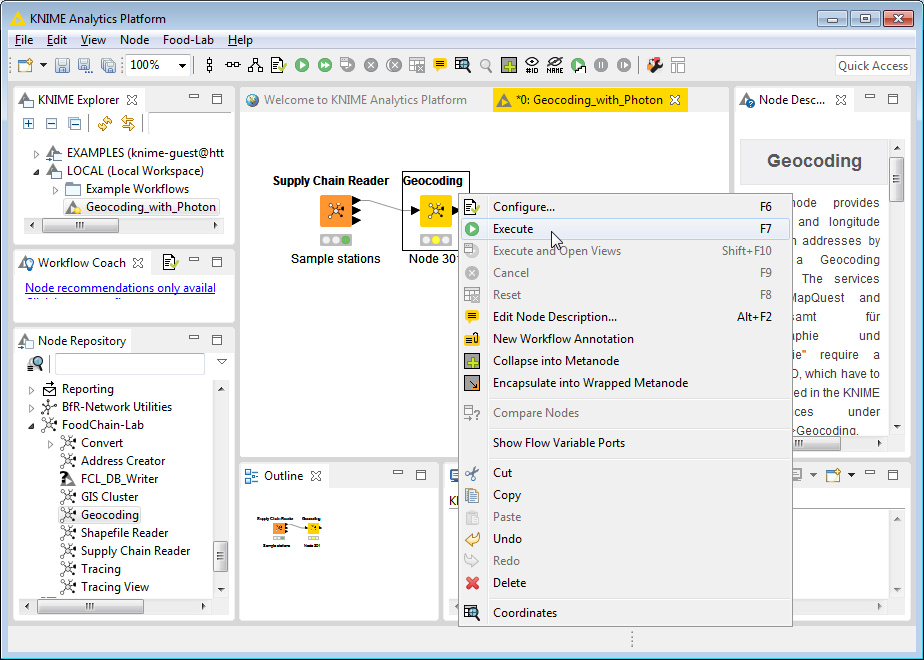
\includegraphics[height=0.6\textheight]{8.png}
	\end{center}
	\begin{itemize}
		\item Die Ausführung kann eine Weile dauern.
		\item Unter dem Knoten wird angezeigt welcher Prozentsatz der Daten bereits bearbeitet wurde.
	\end{itemize}
\end{frame}

\subsection{9}
\begin{frame}
	\begin{center}
  		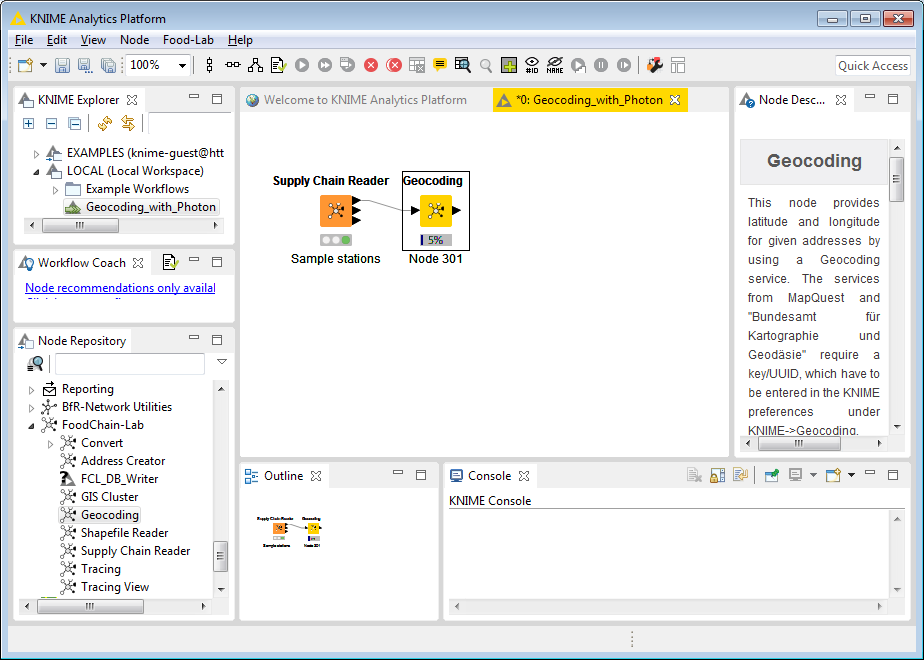
\includegraphics[height=0.6\textheight]{9.png}
	\end{center}
	\begin{itemize}
		\item Wenn die Ausführung beendet ist, können wir uns die Resultate anschauen.
		\item Machen Sie einen Rechtsklick auf den \textbf{Geocoding}-Knoten und wählen Sie \textbf{Coordinates}.
	\end{itemize}
\end{frame}

\subsection{10}
\begin{frame}
	\begin{center}
  		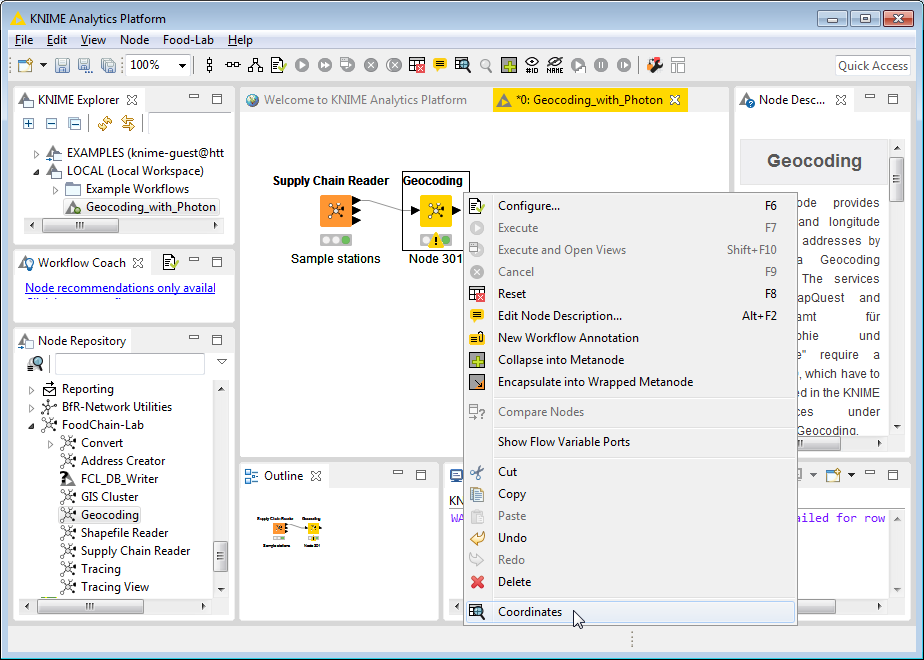
\includegraphics[height=0.6\textheight]{10.png}
	\end{center}
	\begin{itemize}
		\item In dem Dialog können Sie sich die gesamte Datentabelle anschauen.
	\end{itemize}
\end{frame}

\subsection{11}
\begin{frame}
	\begin{center}
  		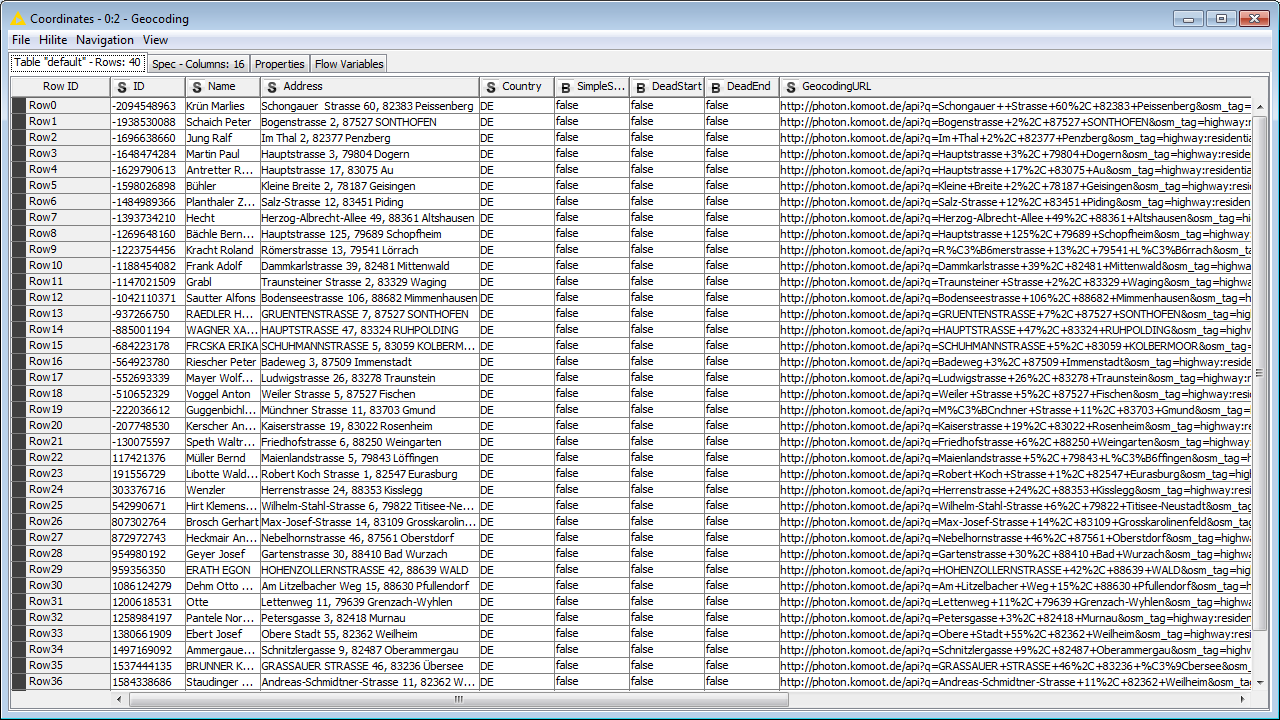
\includegraphics[height=0.6\textheight]{11.png}
	\end{center}
	\begin{itemize}
		\item Scrollen Sie ganz nach rechts um sich die Spalten mit geographischer Breite und Länge anzuschauen (die zwei Spalten ganz rechts).
		\item Eine Geocoding Anfragn lieferte keine Ergebnisse. 
	\end{itemize}
\end{frame}

\end{document}
